% -*- latex -*-
\Level 0 {A style guide for project submissions}

Here are some guidelines for how to submit assignments and projects.
As a general rule, consider programming as an experimental science,
and your writeup as a report on some tests you have done: explain
the problem you're addressing, your strategy, your results.

\paragraph*{\bf Structure of your writeup}

Most of the exercises in this book test whether you are able to code the solution to a certain
problem. That does not mean that turning in the code is sufficient, nor code plus sample output.
Turn in a writeup in pdf form that was generated from a text processing program such as Word or (preferably)
\LaTeX\ (for a tutorial, see~\HPSCref{tut:latex}). Your writeup should have 
\begin{itemize}
\item The relevant fragments of your code,
\item an explanation of your algorithms or solution strategy,
\item a discussion of what you observed,
\item graphs of runtimes and TAU plots; see~\ref{tut:tau}.
\end{itemize}

\paragraph*{Observe, measure, hypothesize, deduce}

In most applications of computing machinery we care about the efficiency with which
we find the solution. Thus, make sure that you do measurements. In general, make
observations that allow you to judge whether your program behaves the way you
would expect it to.

Quite often your program will display unexpected behaviour. It is important to observe
this, and hypothesize what the reason might be for your observed behaviour.

\paragraph*{Including code}

If you include code samples in your writeup, make sure they look good. For starters,
use a mono-spaced font. In \LaTeX, you can use the \n{verbatim} environment or the 
\n{verbatiminput} command. In that section option the source is included automatically,
rather than cut and pasted. This is to be preferred, since your writeup will
stay current after you edit the source file.

Including whole source files makes for a long and boring writeup. The code samples in this
book were generated as follows. In the source files, the relevant snippet was marked as
\begin{verbatim}
... boring stuff
#pragma samplex
  .. interesting! ..
#pragma end
... more boring stuff
\end{verbatim}
The files were then processed with the following command line (actually, included
in a makefile, which requires doubling the dollar signs):
\begin{verbatim}
for f in *.{c,cxx,h} ; do
  cat $x | awk 'BEGIN {f=0}
                   /#pragma end/ {f=0}
                   f==1 {print $0 > file}
                   /pragma/ {f=1; file=$2 }
                '
done
\end{verbatim}
which gives (in this example) a file \n{samplex}. Other solutions are of course possible.

\paragraph*{\bf Code formatting}

Code without proper indentation is very hard to read. Fortunately,
most editors have some knowledge of the syntax of the most popular
languages. The \indexterm{emacs} editor will, most of the time,
automatically activate the appropriate mode based on the file
extension. If this does not happen, you can activate a mode by \n{ESC
  x fortran-mode} et cetera, or by putting the string
\verb+-*- fortran -*-+ in a comment on the first line of your file.

The \indexterm{vi} editor also has syntax support: use the commands
\n{:synxtax on} to get syntax colouring, and \n{:set cindent} to get
automatic indentation while you're entering text. Some of the more
common questions are addressed in
\url{http://stackoverflow.com/questions/97694/auto-indent-spaces-with-c-in-vim}.

\paragraph*{\bf Running your code}

A single run doesn't prove anything. For a good report, you need to
run your code for more than one input dataset (if available) and in
more than one processor configuration. When you choose problem sizes,
be aware that an average processor can do a billion operations per
second: you need to make your problem large enough for the timings to
rise above the level of random variations and startup phenomena.

When you run a code in parallel, beware that on clusters the behaviour
of a parallel code will always be different between one node and
multiple nodes.  On a single node the MPI implementation is likely
optimized to use the shared memory. This means that results obtained
from a single node run will be unrepresentative. In fact, in timing
and scaling tests you will often see a drop in (relative) performance
going from one node to two.  Therefore you need to run your code in a
variety of scenarios, using more than one node.

\paragraph*{Repository organization}

If you submit your work through a repository, make sure you organize your submissions in subdirectories,
and that you give a clear name to all files.

\Level 0 {Warmpup exercises}

We start with some simple exercises.

\Level 1 {Hello world}
\commandrefexercise{sec:rank-size}

First of all we need to make sure that you have a working setup for
parallel jobs. The example program \n{helloworld.c} does the
following:
\verbatimsnippet{hello}
Compile this program and run it in parallel. Make sure that the processors
do \emph{not} all say that they are \n{processor 0 out of 1}!

\begin{istc}
  \Level 1 {Trace output}

  We want to make trace files of the parallel runs, for which we'll
  use the TAU utility of the University of Oregon. 
  (For documentation, go to \url{http://www.cs.uoregon.edu/Research/tau/docs.php}.)
  Here are the steps:
  \begin{itemize}
  \item Load two modules:
\begin{verbatim}
module load tau
module load jdk64
\end{verbatim}
  \item Recompile your program with \n{make yourprog}. You'll notice a
    lot more output: that is the TAU preprocessor.
  \item Now run your program, setting environment variables
    \n{TAU_TRACE} and \n{TAU_PROFILE} to~1, and \n{TRACEDIR} and
    \n{PROFILEDIR} to where you want the output to be.  Big shortcut:
    do 
\begin{verbatim}
make submit EXECUTABLE=yourprog
\end{verbatim}
    for a batch job or 
\begin{verbatim}
make idevrun EXECUTABLE=yourprog
\end{verbatim}
    for an interactive parallel
    run. These last two set all variables for you. See if you can find
    where the output went\ldots
  \item Now you need to postprocess the TAU output. Do \n{make tau
    EXECUTABLE=yourprog} and you'll get a file
    \n{taulog_yourprog.slog2} which you can view with the \n{jumpshot}
    program.
  \end{itemize}
\end{istc}

\Level 1 {Collectives}

It is a good idea to be able to collect statistics, so before we do
anything interesting, we will look at MPI collectives;
section~\ref{sec:collective}.

Take a look at \n{time_max.cxx}. This program sleeps for a random
number of seconds: 
\verbatimsnippet{makejitter}
and measures how long the sleep actually was:
\verbatimsnippet{measurejitter}
In the code, this quantity is called `jitter', which is a term
for random deviations in a system.

\begin{exercise}
  Change this program to compute the average jitter by changing the reduction
  operator.
\end{exercise}

\begin{exercise}
  Now compute the standard deviation
  \[ \sigma = \sqrt{\frac{ \sum_i (x_i-m)^2 }{n} } \]
  where $m$ is the average value you computed in the previous exercise.
  \begin{itemize}
  \item Solve this exercise twice: once by following the reduce by a
    broadcast operation and once by using an \n{Allreduce}.
  \item Run your code both on a single cluster node and on multiple
    nodes, and inspect the TAU trace. Some MPI implementations are
    optimized for shared memory, so the trace on a single node may not
    look as expected.
  \item Can you see from the trace how the allreduce is implemented?
  \end{itemize}
\end{exercise}

\begin{exercise}
  Finally, use a gather call to collect all the values on processor
  zero, and print them out. Is there any process that behaves very
  differently from the others?
\end{exercise}

\begin{istc}
For each exercise, submit code, a TAU trace, and an analysis of what
you see in the traces. Submit your work by leaving a code, graphics,
and a writeup in your repository.
\end{istc}

\Level 1 {Linear arrays of processors}

In this section you are going to write a number of variations on
a very simple operation: 
all processors pass a data item to the processor with the next higher
number.
\begin{itemize}
\item In the file \n{linear-serial.c} you will find an implementation
  using blocking send and receive calls.
\item You will change this code to use non-blocking sends and
  receives; they require an \n{MPI_Wait} call to finalize them.
\item Next, you will use \n{MPI_Sendrecv} to arrive at a synchronous,
  but deadlock-free implementation.
\item Finally, you will use two different one-sided scenarios.
\end{itemize}
In the reference code \n{linear-serial.c}, each process defines two buffers:
\verbatimsnippet{linearnumbers}
where \n{other_number} is the location where the data from the left neighbour is going to be stored.

To check the correctness of the program, there is a gather operation on processor zero:
\verbatimsnippet{serialgathercheck}

\Level 2 {Coding with blocking calls}

Passing data to a neighbouring processor should be a very parallel operation.
However, if we code this naively, with \n{MPI_Send} and \n{MPI_Recv},
we get an unexpected serial behaviour, as was explained in section~\ref{sec:blocking}.
\verbatimsnippet{linear}
(Note that this uses an \n{Ssend}; see section~\ref{sec:handshake}
for the explanation why.)

\begin{exercise}
  Compile and run this code, and generate a TAU trace file. Confirm
  that the execution is serial. Does replacing the \n{Ssend} by \n{Send}
  change this?
\end{exercise}
Let's clean up the code a little.
\begin{exercise}
  First write this code more elegantly by using \n{MPI_PROC_NULL}.
\end{exercise}

\Level 2 {A better blocking solution}

The easiest way to prevent the serialization problem of the previous
exercises is to use the \indexmpishow{MPI_Sendrecv} call. This routine
acknowledges that often a processor will have a receive call whenever there
is a send. For border cases where a send or receive is unmatched you can
use \indexmpishow{MPI_PROC_NULL}.

\begin{exercise}
  Rewrite the code using \n{MPI_Sendrecv}. Confirm with a TAU trace
  that execution is no longer serial.
\end{exercise}

Note that the \n{Sendrecv} call itself is still blocking, but
at least the ordering of its constituent send and recv are
no longer ordered in time.

\Level 2 {Non-blocking calls}

The other way around the blocking behaviour is to use \n{Isend} and \n{Irecv}
calls, which do not block. Of course, now you need a guarantee that these 
send and receive actions are concluded; in this case, use \n{MPI_Waitall}.
\begin{exercise}
  Implement a fully parallel version by using \n{MPI_Isend} and
  \n{MPI_Irecv}.
\end{exercise}

\Level 2 {One-sided communication}

Another way to have non-blocking behaviour is to use one-sided
communication.  During a \n{Put} or \n{Get} operation, execution will
only block while the data is being transferred out of or into the
origin process, but it is not blocked by the target. Again, you need a
guarantee that the transfer is concluded; here use
\indexmpishow{MPI_Win_fence}.

\begin{exercise}
  Write two versions of the code: one using \n{MPI_Put} and one with \n{MPI_Get}.
  Make TAU traces.
\end{exercise}
Investigate blocking behaviour through TAU visualizations. 
\begin{exercise}
  If you transfer a large amount of data, and the target processor is
  occupied, can you see any effect on the origin? Are the fences
  synchronized?
\end{exercise}

\Level 0 {Mandelbrot set}

If you've never heard the name \indexterm{Mandelbrot set}, you
probably recognize the picture. Its formal definition is as follows:
\begin{quotation}\noindent
  A point $c$ in the complex plane is part of the Mandelbrot set if 
  the series $x_n$ defined by 
  \[ 
  \begin{cases}
    x_0=0\\ x_{n+1}=x_n^2+c
  \end{cases}
  \] satisfies \[ \forall_n\colon |x_n|\leq 2. \]  
\end{quotation}
It is easy to see that only points $c$ in the bounding circle
$|c|< 2$ qualify, but
apart from that it's hard to say much without a lot more thinking.
Or computing; and that's what we're going to do.

In this set of exercises you are going to take an example program
\n{mandel_main.cxx} and extend it to use a variety of MPI programming
constructs.  This program has been set up as a
\indexterm{master-worker} model: there is one master processor (for a
change this is the last processor, rather than zero) which gives out
work to, and accepts results from, the worker processors. It then
takes the resuls and construct an image file from them.

\Level 1 {Invocation}

The \n{mandel_main} program is called as
\begin{verbatim}
mpirun -np 123 mandel_main steps 456 iters 789
\end{verbatim}
where the \n{steps} parameter indicates how many steps in $x,y$
direction there are in the image, and \n{iters} gives the maximum
number of iterations in the \n{belong} test.

If you forget the parameter, you can call the program with
\begin{verbatim}
mandel_serial -h
\end{verbatim}
and it will print out the usage information.

\Level 1 {Tools}

The driver part of the Mandelbrot program is simple. There is a 
circle object that can generate coordinates
\verbatimsnippet{circledef}
and a global routine that tests whether a coordinate is in the set,
at least up to an iteration bound. It returns zero if the 
series from the given starting point has not diverged,
or the iteration number in which it diverged if it did so.
\verbatimsnippet{belongs}
In the former case,  the point could be in the Mandelbrot set, 
and we colour it black, in the latter case we give it a colour
depending on the iteration number.
\verbatimsnippet{pickcolour}
We use a fairly simple code for the worker processes: they 
execute a loop in which they wait 
for input, process it, return the result.
\verbatimsnippet{waitforwork}

A very simple solution using blocking sends on the master is given:
\verbatimsnippet{serialaddtask}

\begin{exercise}
  Explain why this solution is very inefficient. Make a trace of its
  execution that bears this out.
\end{exercise}

\Level 1 {Bulk task scheduling}
\label{proj:mandel-bulk}

The previous section showed a very inefficient solution, but that was mostly
intended to set up the code base. If all tasks take about the same amount of time,
you can give each process a task, and then wait on them all to finish. A~first way
to do this is with non-blocking sends.

\begin{exercise}
  Code a  solution where you give a task to all worker processes
  using non-blocking sends and receives, and then wait for these tasks
  with \n{MPI_Waitall}
  to finish before you give a new round of data to all workers.
  Make a trace of the execution of this and report on the total time.

  You can do this by writing a new class that inherits from \n{queue},
  and that provides its own \n{addtask} method:
\verbatimsnippet{bulkq}
  You will also have to override the \n{complete} method: when the circle 
  object indicates that all coordinates have been generated, not all
  workers will be busy, so you need to supply the proper \n{MPI_Waitall}
  call.
\end{exercise}

\Level 1 {Collective task scheduling}
\label{proj:mandel-collective}

Another implementation of the bulk scheduling of the previous section
would be through using collectives.

\begin{exercise}
  Code a solution which uses scatter to distribute data to the worker
  tasks, and gather to collect the results. Is this solution more or
  less efficient than the previous?
\end{exercise}

\Level 1 {Asynchronous task scheduling}

At the start of section~\ref{proj:mandel-bulk} we said that bulk scheduling
mostly makes sense if all tasks take similar time to complete.
In the Mandelbrot case this is clearly not the case.

\begin{exercise}
  Code a fully dynamic solution that uses \n{MPI_Probe} or \n{MPI_Waitany}.
  Make an execution trace and report on the total running time.
\end{exercise}

\Level 1 {One-sided solution}

Let us reason about whether it is possible (or advisable) to code a
one-sided solution to computing the Mandelbrot set.  
%
With active
target synchronization you could have an exposure window on the host
to which the worker tasks would write. To prevent conflicts you would allocate an 
array and have each worker write to a separate location in it.
%
The problem here is that the workers may not be sufficiently synchronized because
of the differing time for computation.

Consider then passive target synchronization. Now the worker tasks could
write to the window on the master whenever they have something to
report; by locking the window they prevent other tasks from interfering.
%
After a worker writes a result, it can get new data from an array
of all coordinates on the master. 

It is hard to get results into the image as they become available. For
this, the master would continuously have to scan the results
array. Therefore, constructing the image is easiest done when all
tasks are concluded.

\Level 0 {Data parallel grids}

\Level 1 {A realistic programming example}

In this section we will gradually build a semi-realistic example
program. To get you started some pieces have already been written:
as a starting point look at \n{code/mpi/c/grid.cxx}.

\Level 2 {Description of the problem}

With this example you will investigate several strategies for
implementing a simple iterative method. Let's say you have a
two-dimensional grid of datapoints $G=\{g_{ij}\colon 0\leq
i<n_i,\,0\leq j<n_j\}$ and you want to compute~$G'$ where
\begin{equation}
g'_{ij} = 1/4 \cdot (g_{i+1,j}+g_{i-1,j}+g_{i,j+1}+g_{i,j-1}).
\label{eq:grid-update}
\end{equation}

This is easy enough to implement sequentially, but in parallel this
requires some care.

Let's divide the grid $G$ and divide it over a two-dimension grid of
$p_i\times p_j$
processors. (Other strategies exist, but this one scales best; see
section~\HPSCref{sec:pspmvp}.)
Formally, we define two sequences of points
\[ 0=i_0<\cdots<i_{p_i}<i_{p_i+1}=n_i,\quad 
   0<j_0<\cdots<j_{p_j}<i_{p_j+1}=n_j
\]
and we say that processor $(p,q)$ computes $g_{ij}$ for
\[ i_p\leq i<i_{p+1}, \quad j_q\leq j<j_{q+1}.
\]
From formula~\eqref{eq:grid-update} you see that the processor then
needs one row of points on each side surrounding its part of the
grid. A~picture makes this clear; see figure~\ref{fig:ghost-grid}.
\begin{figure}
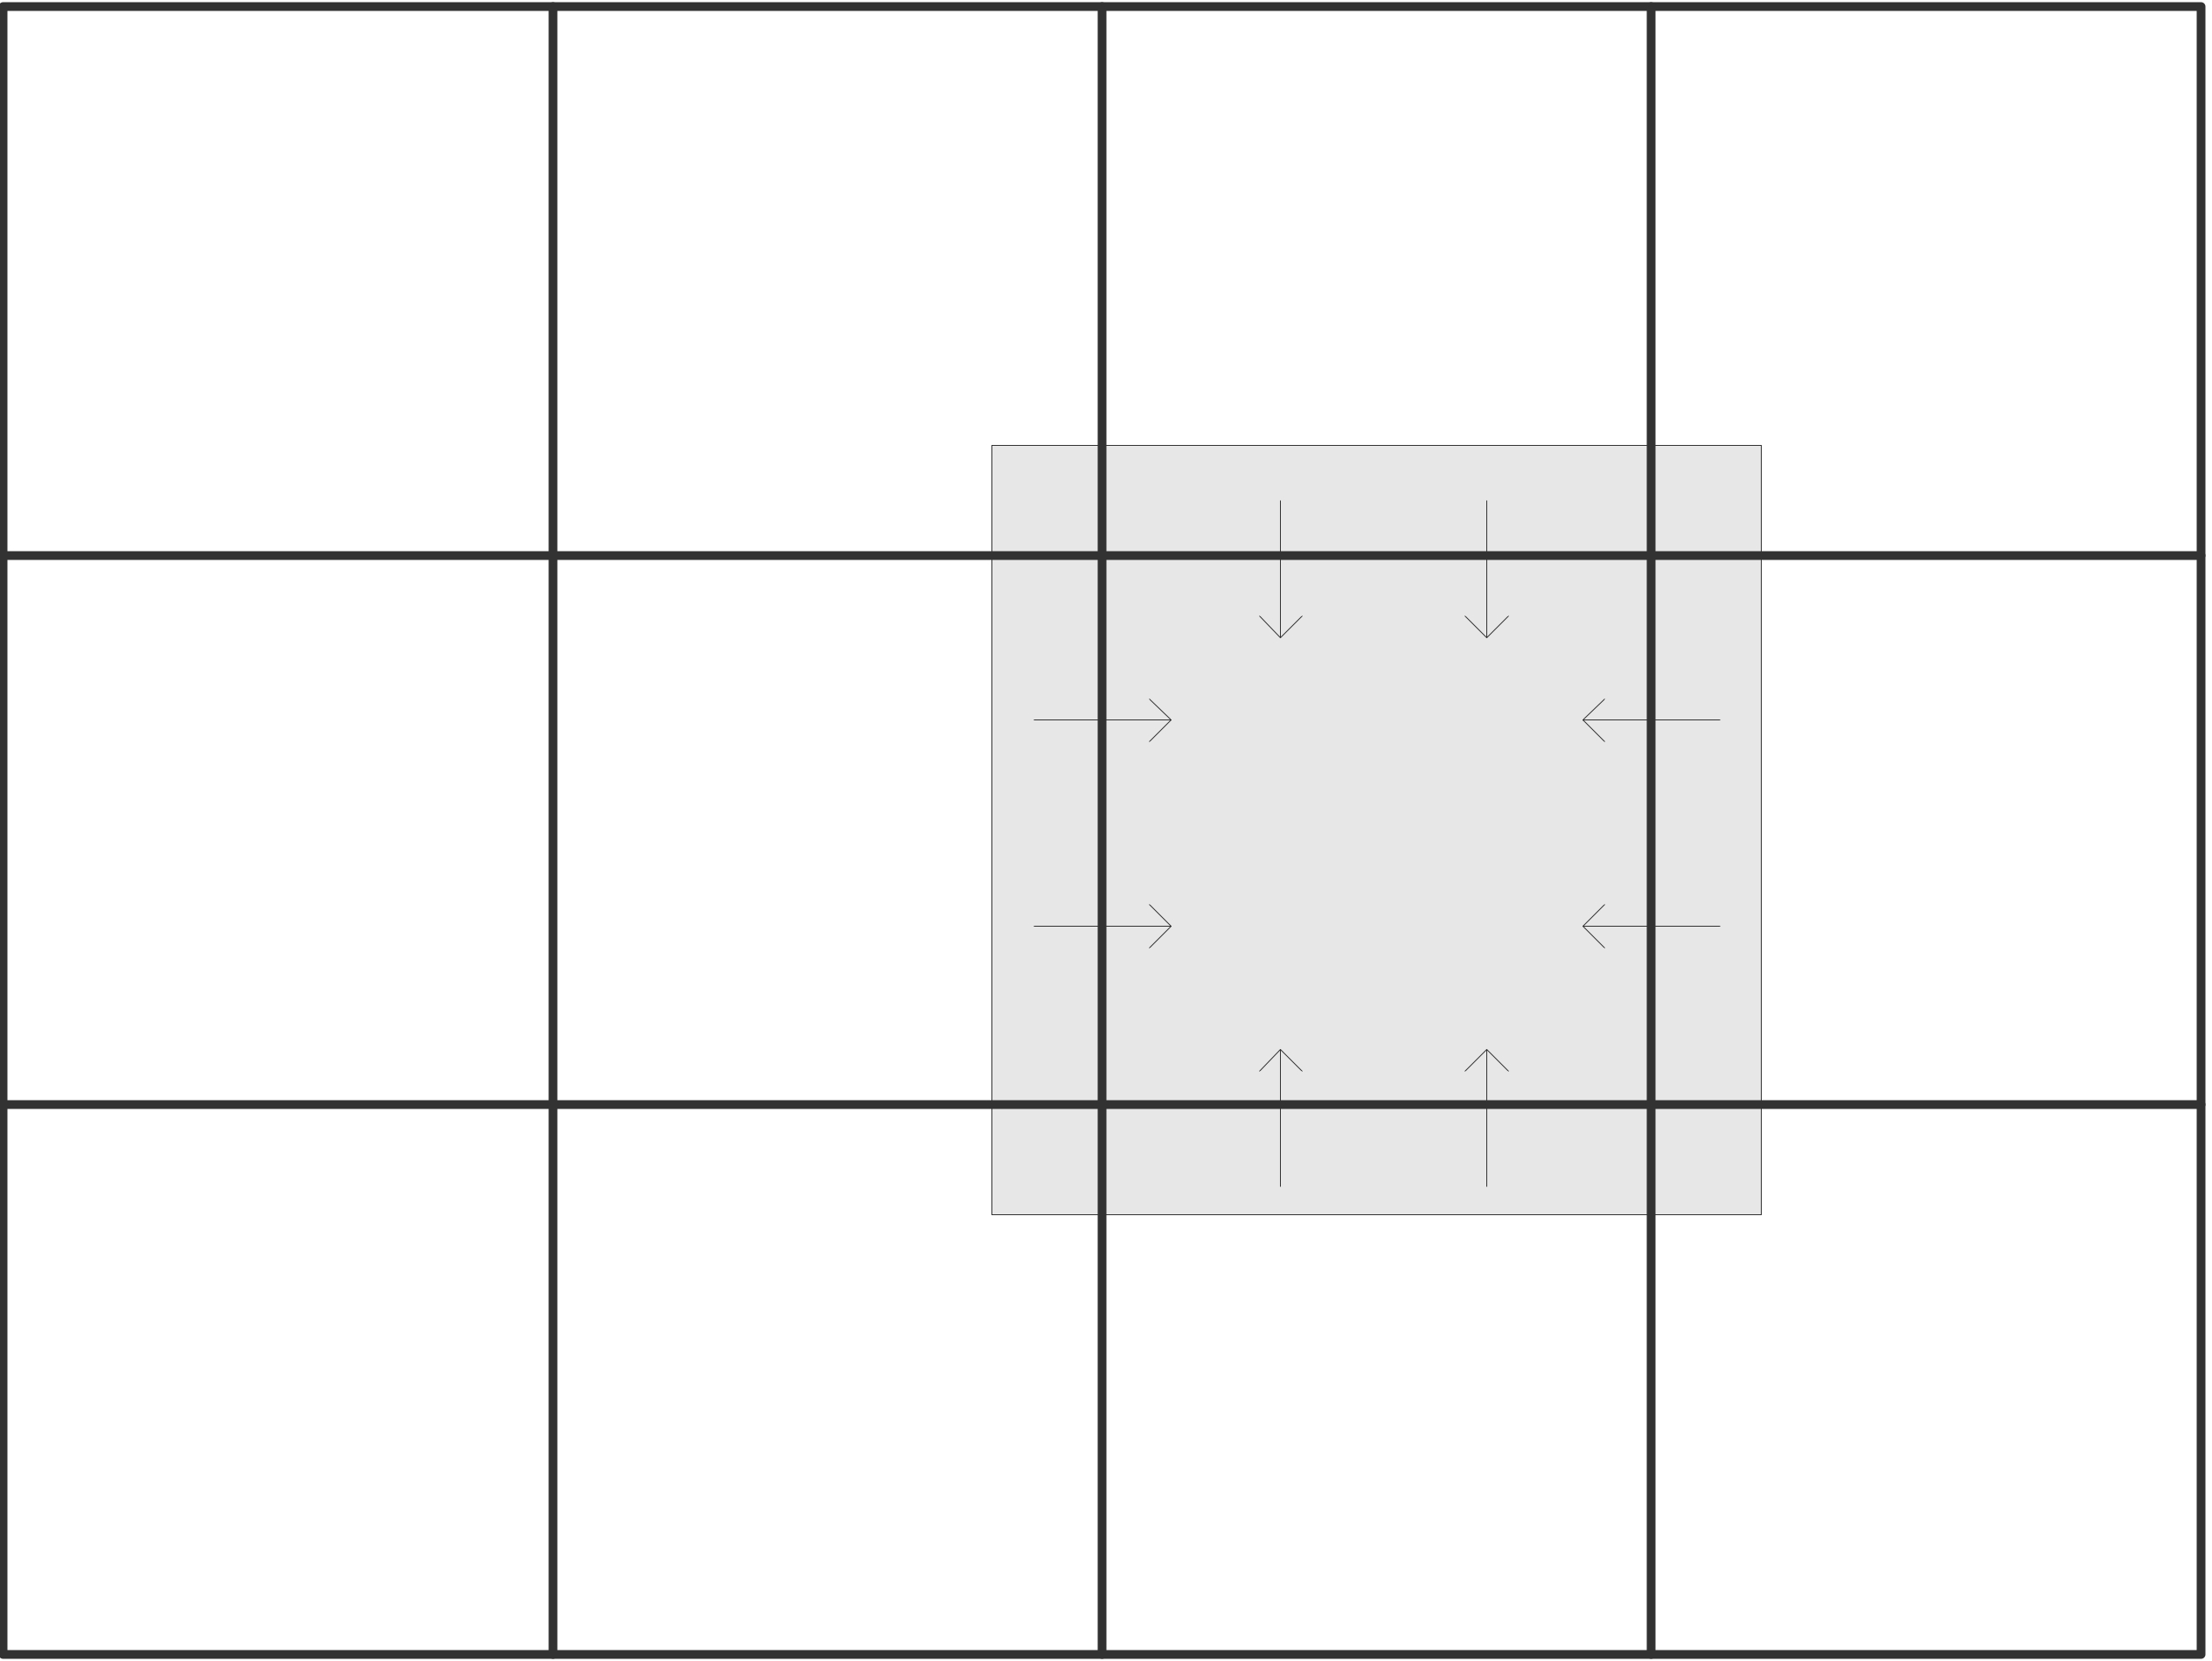
\includegraphics[scale=.1]{graphics/jacobi-average}
\caption{A grid divided over processors, with the `ghost' region indicated}
\label{fig:ghost-grid}
\end{figure}
These elements surrounding the processor's own part are called
the \indexterm{halo} or \indexterm{ghost region} of that processor.

The problem is now that the elements in the halo are stored on a
different processor, so communication is needed to gather them. In the
upcoming exercises you will have to use different strategies for doing
so.

\Level 2 {Code basics}

The program needs to read the values of the grid size and the
processor grid size from the commandline, as well as the number of
iterations. This routine does some error checking: if the number of
processors does not add up to the size of \n{MPI_COMM_WORLD}, a
nonzero error code is returned.
\begin{verbatim}
ierr = parameters_from_commandline
  (argc,argv,comm,&ni,&nj,&pi,&pj,&nit);
if (ierr) return MPI_Abort(comm,1);
\end{verbatim}
From the processor parameters we make a processor grid object:
\begin{verbatim}
processor_grid *pgrid = new processor_grid(comm,pi,pj);
\end{verbatim}
and from the numerical parameters we make a number grid:
\begin{verbatim}
number_grid *grid = new number_grid(pgrid,ni,nj);
\end{verbatim}
Number grids have a number of methods defined. To set the value of all
the elements belonging to a processor to that processor's number:
\begin{verbatim}
grid->set_test_values();
\end{verbatim}
To set random values:
\begin{verbatim}
grid->set_random_values();
\end{verbatim}
If you want to visualize the whole grid, the following call gathers
all values on processor zero and prints them:
\begin{verbatim}
grid->gather_and_print();
\end{verbatim}

Next we need to look at some data structure details.

The definition of the \n{number_grid} object starts as follows:
\begin{verbatim}
class number_grid {
public:
  processor_grid *pgrid;
  double *values,*shadow;
\end{verbatim}
where \n{values} contains the elements owned by the processor,
and \n{shadow} is intended to contain the values plus the ghost
region. So how does \n{shadow} receive those values? Well, the call looks 
like
\begin{verbatim}
grid->build_shadow();
\end{verbatim}
and you will need to supply the implementation of that.
Once you've done so, there is a routine that prints out the shadow array 
of each processor
\begin{verbatim}
grid->print_shadow();
\end{verbatim}
This routine does the sequenced printing that you implemented in
exercise~\ref{ex:hello-world-zero}.

In the file \n{code/mpi/c/grid_impl.cxx} you can see several uses of
the macro \n{INDEX}. This translates from a two-dimensional coordinate
system to one-dimensional. Its main use is letting you use $(i,j)$
coordinates for indexing the processor grid and the number grid: for
processors you need the translation to the linear rank, and for the
grid you need the translation to the linear array that holds the
values.

A good example of the use of \n{INDEX} is in the
\n{number_grid::relax} routine: this takes points from the \n{shadow}
array and averages them into a point of the \n{values} array. (To
understand the reason for this particular averaging,
see~\HPSCref{sec:2dbvp} and~\HPSCref{sec:jacobi-seidel}.) Note how the
\n{INDEX} macro is used to index in a
$\n{ilength}\times\n{jlength}$ target array \n{values}, while
reading from a $(\n{ilength}+2)\times(\n{jlength}+2)$ source array
\n{shadow}.
\begin{verbatim}
for (i=0; i<ilength; i++) {
  for (j=0; j<jlength; j++) {
    int c=0;
    double new_value=0.;
    for (c=0; c<5; c++) {
	int ioff=i+1+ioffsets[c],joff=j+1+joffsets[c];
	new_value += coefficients[c] * 
	  shadow[ INDEX(ioff,joff,ilength+2,jlength+2) ];
    }
    values[ INDEX(i,j,ilength,jlength) ] = new_value/8.;
  }
}
\end{verbatim}

